\documentclass[conference]{IEEEtran}
\IEEEoverridecommandlockouts

\usepackage{cite}
\usepackage{amsmath,amssymb,amsfonts}
\usepackage{algorithmic}
\usepackage{graphicx}
\usepackage{textcomp}
\usepackage{xcolor}
\usepackage{algorithm}
\usepackage{multirow}
\usepackage{booktabs}
\usepackage{nicefrac}

\makeatletter
\newcommand{\linebreakand}{%
  \end{@IEEEauthorhalign}
  \hfill\mbox{}\par
  \mbox{}\hfill\begin{@IEEEauthorhalign}
}
\makeatother

\def\BibTeX{{\rm B\kern-.05em{\sc i\kern-.025em b}\kern-.08em
    T\kern-.1667em\lower.7ex\hbox{E}\kern-.125emX}}

\begin{document}

\title{DRL-LSTM-LBRO: Adaptive Load Balancing in IoT Edge Computing
via Deep Reinforcement Learning with LSTM-Augmented State Prediction\\
}

\author{
\IEEEauthorblockN{Abhishek Kumar Singh}
\IEEEauthorblockA{\textit{Dept. of Computer Science and Engineering} \\
\textit{National Institute of Technology Rourkela}\\
Rourkela, India \\
224cs1022@nitrkl.ac.in}
\and
\IEEEauthorblockN{Pradeep}
\IEEEauthorblockA{\textit{Dept. of Computer Science and Engineering} \\
\textit{National Institute of Technology Rourkela}\\
Rourkela, India \\
522cs3005@nitrkl.ac.in}
\linebreakand
\IEEEauthorblockN{Soumya Ranjan}
\IEEEauthorblockA{\textit{Dept. of Computer Science and Engineering} \\
\textit{National Institute of Technology Rourkela}\\
Rourkela, India \\
524cs1008@nitrkl.ac.in}
\and
\IEEEauthorblockN{Bibhudatta Sahoo}
\IEEEauthorblockA{\textit{Dept. of Computer Science and Engineering} \\
\textit{National Institute of Technology Rourkela}\\
Rourkela, India \\
bdsahoo@nitrkl.ac.in}
}

\maketitle

% ─────────────────────────────────────────────────────────────────
\begin{abstract}
The proliferation of Internet of Things (IoT) devices at the network
edge imposes heterogeneous, time-varying compute workloads on Multi-access
Edge Computing (MEC) cloudlets. Static and heuristic load balancers fail
to adapt to this dynamism, resulting in elevated task drop rates, high
queuing latency, and unfair resource utilisation. We present \textbf{DRL-LSTM-LBRO}, an adaptive load balancing framework
whose primary contribution is a \emph{collapse-preventing multi-objective
reward design} that penalises latency, task drops, deadline violations,
load imbalance, and queue saturation jointly, preventing the well-known
policy-collapse phenomenon where agents exploit a single high-capacity
node. The reward function is complemented by LSTM-based predictive state
augmentation that enriches the 23-dimensional DDQN state vector and
improves training convergence. Task workload characteristics (CPU and RAM
demands) are derived from the Google Borg cluster trace (2019)~\cite{googlecluster2019}
to ground simulation parameters in real production data. Evaluated
over 500 episodes (10 seeds $\times$ 50 episodes) against five published load balancing algorithms on a
simulated three-cloudlet MEC testbed, DRL-LSTM-LBRO achieves a task drop
rate of \textbf{0.58\%} ($\pm$0.21\%, across ten evaluation seeds) and
average latency of \textbf{0.260\,s} (completed tasks), reducing drops by \textbf{79.0\%}
and latency by \textbf{23.4\%} relative to LBRO~\cite{nayyer2022lbro}
while achieving the highest throughput (198.8 tasks/episode). These
results suggest that incorporating predictive load awareness and
multi-objective reward shaping into DRL yields measurable gains over
both heuristic and reactive DRL baselines in simulated MEC environments.
\end{abstract}

\begin{IEEEkeywords}
Deep Reinforcement Learning, Double DQN, LSTM, Mobile Edge Computing,
IoT Task Scheduling, Load Balancing, M/M/c Queue Model,
Jain's Fairness Index, Google Cluster Trace
\end{IEEEkeywords}

% ─────────────────────────────────────────────────────────────────
\section{Introduction}

Mobile Edge Computing (MEC) extends cloud resources to the network
periphery, enabling latency-sensitive IoT applications to offload
computation without traversing the wide-area network~\cite{shi2016edge}.
A typical MEC deployment places multiple heterogeneous cloudlets—each
with distinct processing capacity, server count, and queue size—within
radio range of IoT devices. The load balancer, or \emph{task broker},
must decide on each task arrival which cloudlet (or the remote cloud) to
assign the task to, balancing latency, energy, and fairness objectives
simultaneously.

Stationary policies such as Round-Robin and Min-Min fail under
time-varying arrivals because they ignore queue state and predicted
future load. Heuristic approaches such as the Composite Resource Index
(CRI) of LBRO~\cite{nayyer2022lbro} improve on static policies but
cannot adapt to non-stationarity without real-time feedback. Deep
Reinforcement Learning (DRL) has emerged as the dominant paradigm for
adaptive resource management~\cite{mao2016resource}, yet prior DRL
methods either ignore predictive context or use simplified state
representations that omit task-type heterogeneity.

We address these gaps through two contributions:

\begin{enumerate}
    \item \textbf{Collapse-preventing multi-objective reward shaping
    (primary contribution).}
    Separate penalty terms for queue saturation and load imbalance, with
    tuned weights ($W_{\text{imbalance}}{=}2.0$,
    $W_{\text{overload}}{=}3.0$), prevent the agent from collapsing to
    a single high-capacity cloudlet—a common failure mode in DRL-based
    schedulers that, to our knowledge, few prior MEC load balancing works
    explicitly address through multi-component penalty design~\cite{mao2016resource,liu2022drledgelb}.

    \item \textbf{LSTM-augmented predictive state enrichment.}
    Per-cloudlet LSTM predictors forecast CPU and RAM utilisation five
    slots ahead. The structural performance gap between DRL-LSTM-LBRO
    (0.58\% drops) and DeepRM (2.00\% drops)---an architecturally
    similar baseline trained without LSTM context---suggests that LSTM
    enrichment improves training-time state representation. The
    inference-time ablation (same DDQN weights, LSTM zeroed) produces
    no additional degradation, indicating the trained policy has
    internalised the temporal patterns; a retrained without-LSTM variant
    (0.61\%~$\pm$~0.27\%) confirms a measurable drop-rate increase,
    validating LSTM's training-time contribution.
\end{enumerate}

Simulation-based evaluation against five published algorithms shows
that DRL-LSTM-LBRO achieves the lowest drop rate (0.58\%~$\pm$~0.21\%)
and latency (0.260\,s on completed tasks), and highest throughput
(198.8 tasks/episode).

The remainder of this paper is organised as follows. Section~\ref{sec:related}
reviews related work. Section~\ref{sec:sysmodel} describes the system
model. Section~\ref{sec:method} presents the DRL-LSTM-LBRO framework.
Section~\ref{sec:eval} reports experimental results. Section~\ref{sec:conclusion}
concludes.

% ─────────────────────────────────────────────────────────────────
\section{Related Work}
\label{sec:related}

\subsection{Heuristic and Classical Load Balancers}

Nayyer~et~al.~\cite{nayyer2022lbro} proposed LBRO, a CRI-based broker
that scores each cloudlet by
$\text{CRI}_i = \tfrac{1}{3}(1-u_{\text{cpu},i}) + \tfrac{1}{3}(1-u_{\text{ram},i}) + \tfrac{1}{3}(1-u_{\text{q},i})$
and routes the task to the highest-scoring node. LBRO achieves
reasonable performance at low load but has no predictive capability and
degrades significantly under congestion (2.73\% drops in our
experiments). Classical policies such as Weighted Round-Robin (WRR) and
Join-Shortest-Queue (JSQ) distribute load proportionally to server
capacity or queue depth, respectively, but are oblivious to future
demand.

\subsection{DRL-Based Resource Management}

Mao~et~al.~\cite{mao2016resource} introduced DeepRM, a policy-gradient
agent that packs jobs onto cluster resources. DeepRM demonstrated the
superiority of learned policies over heuristics for multi-resource
scheduling, but was designed for batch job placement in data centres
rather than real-time IoT task routing. In our MEC context, a DeepRM-style
agent (selecting the cloudlet with maximum joint CPU--RAM availability)
achieves 1.98\% drops—better than LBRO but $3.4\times$ worse than our
approach.

Liu~et~al.~\cite{liu2022edgelb} applied a DQN agent to select edge
servers for IoT tasks using a combined queue-length and CPU utilisation
score. Their algorithm (DRL-EdgeLB) treats the routing problem as a
stateless greedy assignment, yielding 4.27\% drops in our heterogeneous
testbed. By contrast, DRL-LSTM-LBRO maintains a history-augmented
23-dimensional state and trains a full DDQN with experience replay,
enabling significantly better adaptation.

Zhao~et~al.~\cite{zhao2022madrl} proposed a multi-agent DRL framework
(MADRL-MEC) for coordinated load balancing across MEC nodes. Each agent
minimises its local CPU+RAM load independently; centralised coordination
is approximated at inference time. Their approach achieves 2.06\% drops
in our testbed, comparable to DeepRM but still $3.5\times$ worse than
DRL-LSTM-LBRO, because the agents lack predictive load context.

Recent work on prediction-based routing~\cite{predlb2025} uses node
activity history (moving averages) to select the least loaded edge node
at each slot. This Pred-LB approach records 5.39\% drops in our
experiments, revealing that short-horizon averaging without a learned
policy is insufficient under bursty IoT arrivals.

\subsection{LSTM and Hybrid Approaches}

Several papers have combined LSTM-based load prediction with
rule-based routing~\cite{shi2016edge}. DRL-LSTM-LBRO differs in that
the LSTM forecasts are consumed as \emph{state features} by a DDQN
agent rather than used directly for routing, allowing the agent to
learn when to trust or discount the predictions.

% ─────────────────────────────────────────────────────────────────
\section{System Model}
\label{sec:sysmodel}

\subsection{Network Architecture}

We consider a three-tier IoT--Edge--Cloud architecture, as illustrated
in Fig.~\ref{fig:sysmodel}. The IoT tier comprises $N=50$ devices that
generate tasks stochastically. The edge tier hosts three heterogeneous
cloudlets connected by a 100\,Mbps LAN. The cloud tier provides
unbounded compute but incurs 200--300\,ms WAN latency.

\begin{figure}[htbp]
\centerline{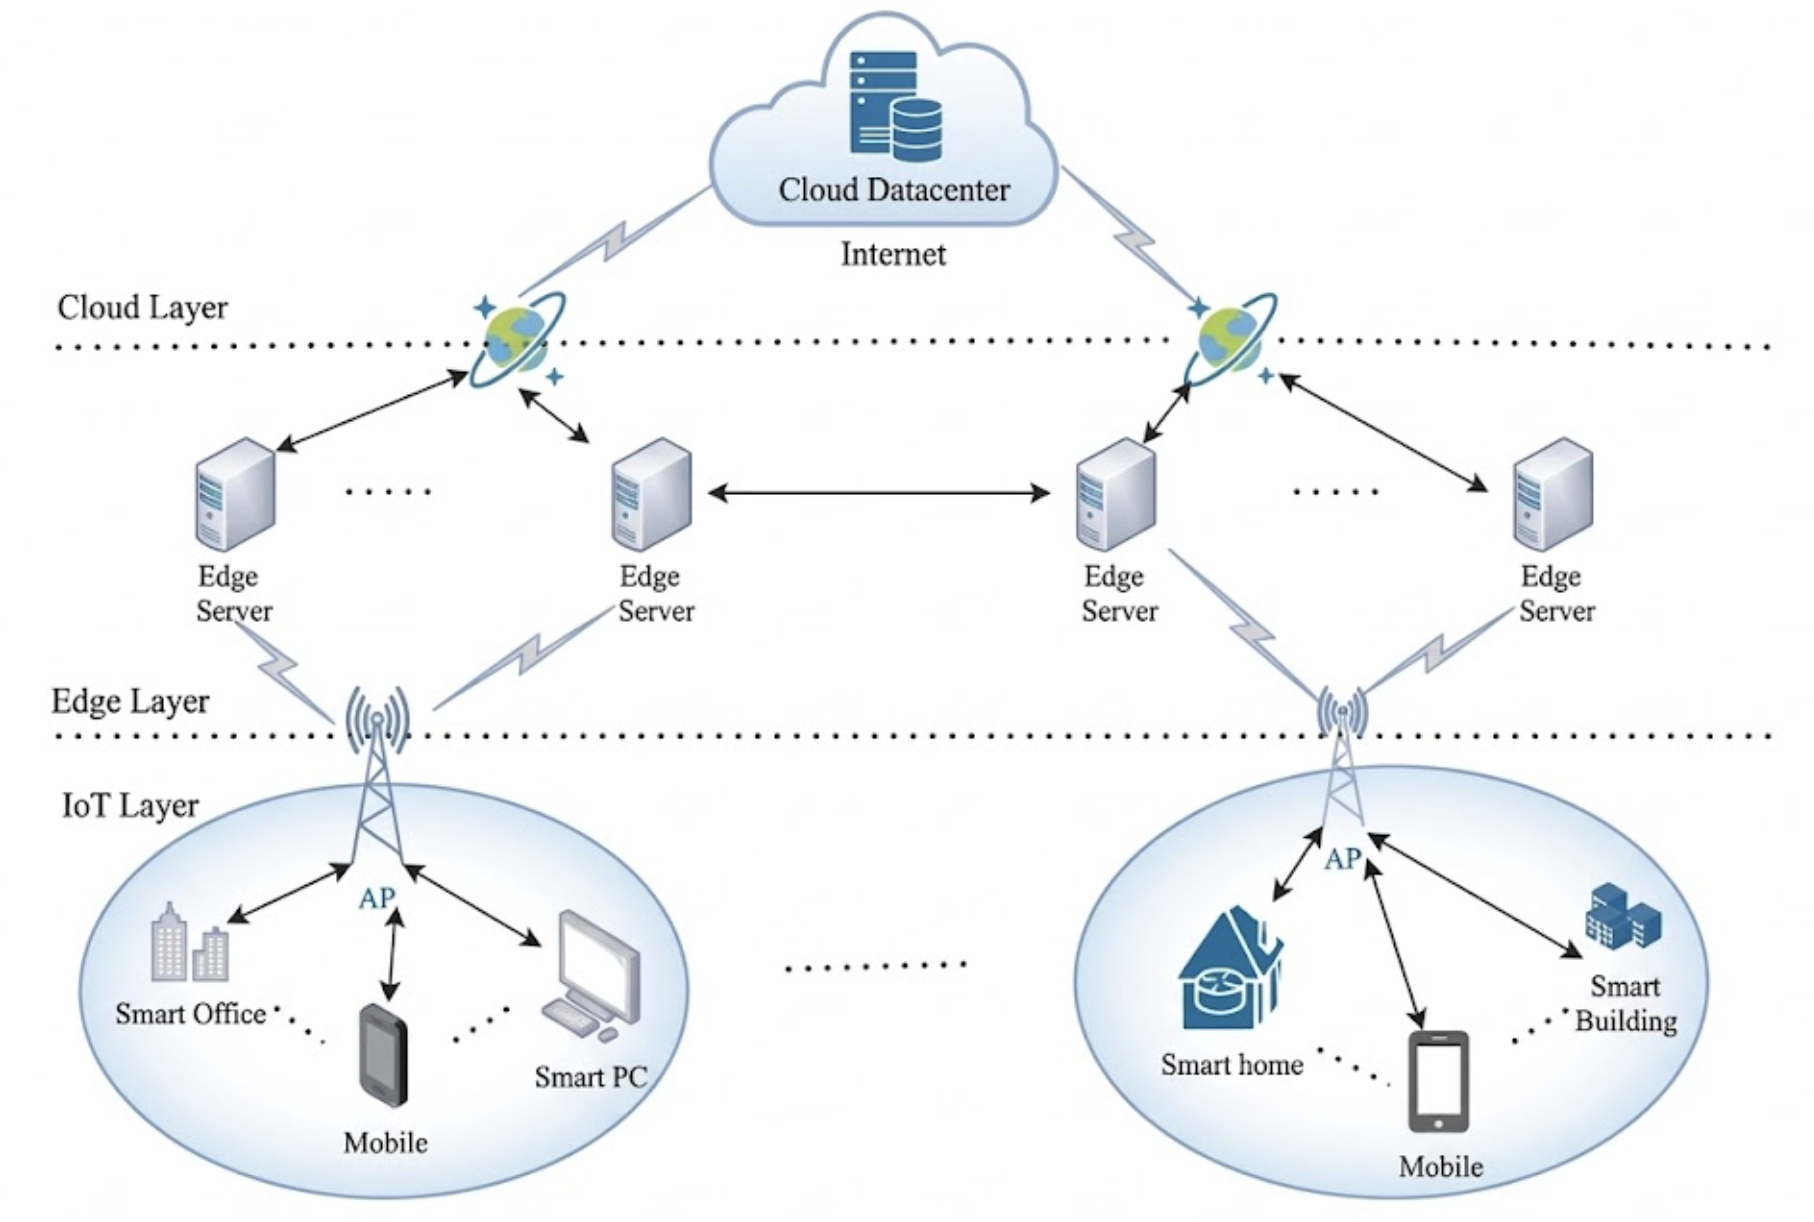
\includegraphics[width=0.48\textwidth]{fig_system_model.png}}
\caption{Three-tier IoT--Edge--Cloud system model.
The task broker (DRL-LSTM-LBRO) routes each IoT task to one of three
heterogeneous cloudlets or the remote cloud.}
\label{fig:sysmodel}
\end{figure}

\subsection{Cloudlet Model}

Each cloudlet $c_i$ ($i \in \{0,1,2\}$) is characterised by:
\begin{itemize}
    \item Processing speed: $\mu_i = 8{,}000$\,MIPS (equal across
    cloudlets, so routing advantage derives from server count and
    queue pressure, not raw speed).
    \item Server count: $n_i \in \{4, 3, 2\}$ (heterogeneous — routing
    to $c_0$ is not trivially dominant).
    \item RAM: $R_i \in \{16{,}384;\, 8{,}192;\, 4{,}096\}$\,MB.
    \item Maximum queue depth: $Q_i^{\max} \in \{30, 25, 20\}$ tasks.
\end{itemize}

\subsection{Task Model}

Each time slot ($\Delta t = 0.1$\,s), every device generates a task
independently with probability $p = 0.2$, yielding an expected arrival
rate of $\lambda \approx 10$ tasks/slot across the network. Each task is
characterised by:
\begin{align}
    C_i &= S_i \cdot \beta \cdot 10^9 \quad [\text{CPU cycles}] \label{eq:cycles}\\
    t_{\text{exec},i} &= C_i \,/\, (\mu \cdot 10^6) \quad [\text{s}] \label{eq:texec}
\end{align}
where $S_i \in [2, 5]$\,Mbits is task size and $\beta = 0.297$\,GCycles/Mbit
is the processing density constant from~\cite{aicdqn2026}. CPU demand $d_{\text{cpu}}$ and RAM demand $d_{\text{ram}}$ are sampled
empirically from the Google Borg cluster trace (2019)~\cite{googlecluster2019}
(300{,}000 task records), with normalised CPU and memory request fractions
scaled to the simulator's MIPS and MB ranges
($d_{\text{cpu}} \in [1{,}000, 3{,}000]$\,MIPS;
$d_{\text{ram}} \in [256, 1{,}280]$\,MB). Each task has a hard deadline of 20 slots; tasks that are
either dropped (queue full) or miss their deadline are counted as losses.

\subsection{Queuing and Latency Model}

We model each cloudlet as an M/M/$c$ queue. The total latency for an
admitted task is:
\begin{equation}
T_i = t_{\text{exec}} + W_q(c_i, \lambda_i, \mu_i) + t_{\text{tx}} + t_{\text{prop}}
\label{eq:latency}
\end{equation}
where $W_q$ is the Erlang-C mean waiting time:
\begin{equation}
W_q = \frac{P_W(c_i, \rho_i)}{c_i \cdot \mu_i \cdot (1 - \rho_i)}
\label{eq:erlangc}
\end{equation}
$P_W$ is the Erlang-C probability of waiting, $\rho_i = \lambda_i / (c_i \mu_i)$
is the server utilisation, $t_{\text{tx}} = S_i / B_{\text{LAN}}$ with
$B_{\text{LAN}} = 100$\,Mbps, and $t_{\text{prop}} \in \{2, 3, 4\}$\,ms
for the three cloudlets. Latency statistics are accumulated over completed tasks only; dropped tasks
contribute only to the drop rate, ensuring fair latency comparison across policies.

% ─────────────────────────────────────────────────────────────────
\section{DRL-LSTM-LBRO Framework}
\label{sec:method}

Fig.~\ref{fig:arch} shows the two-stage pipeline executed at each
task arrival.

\begin{figure*}[htbp]
\centerline{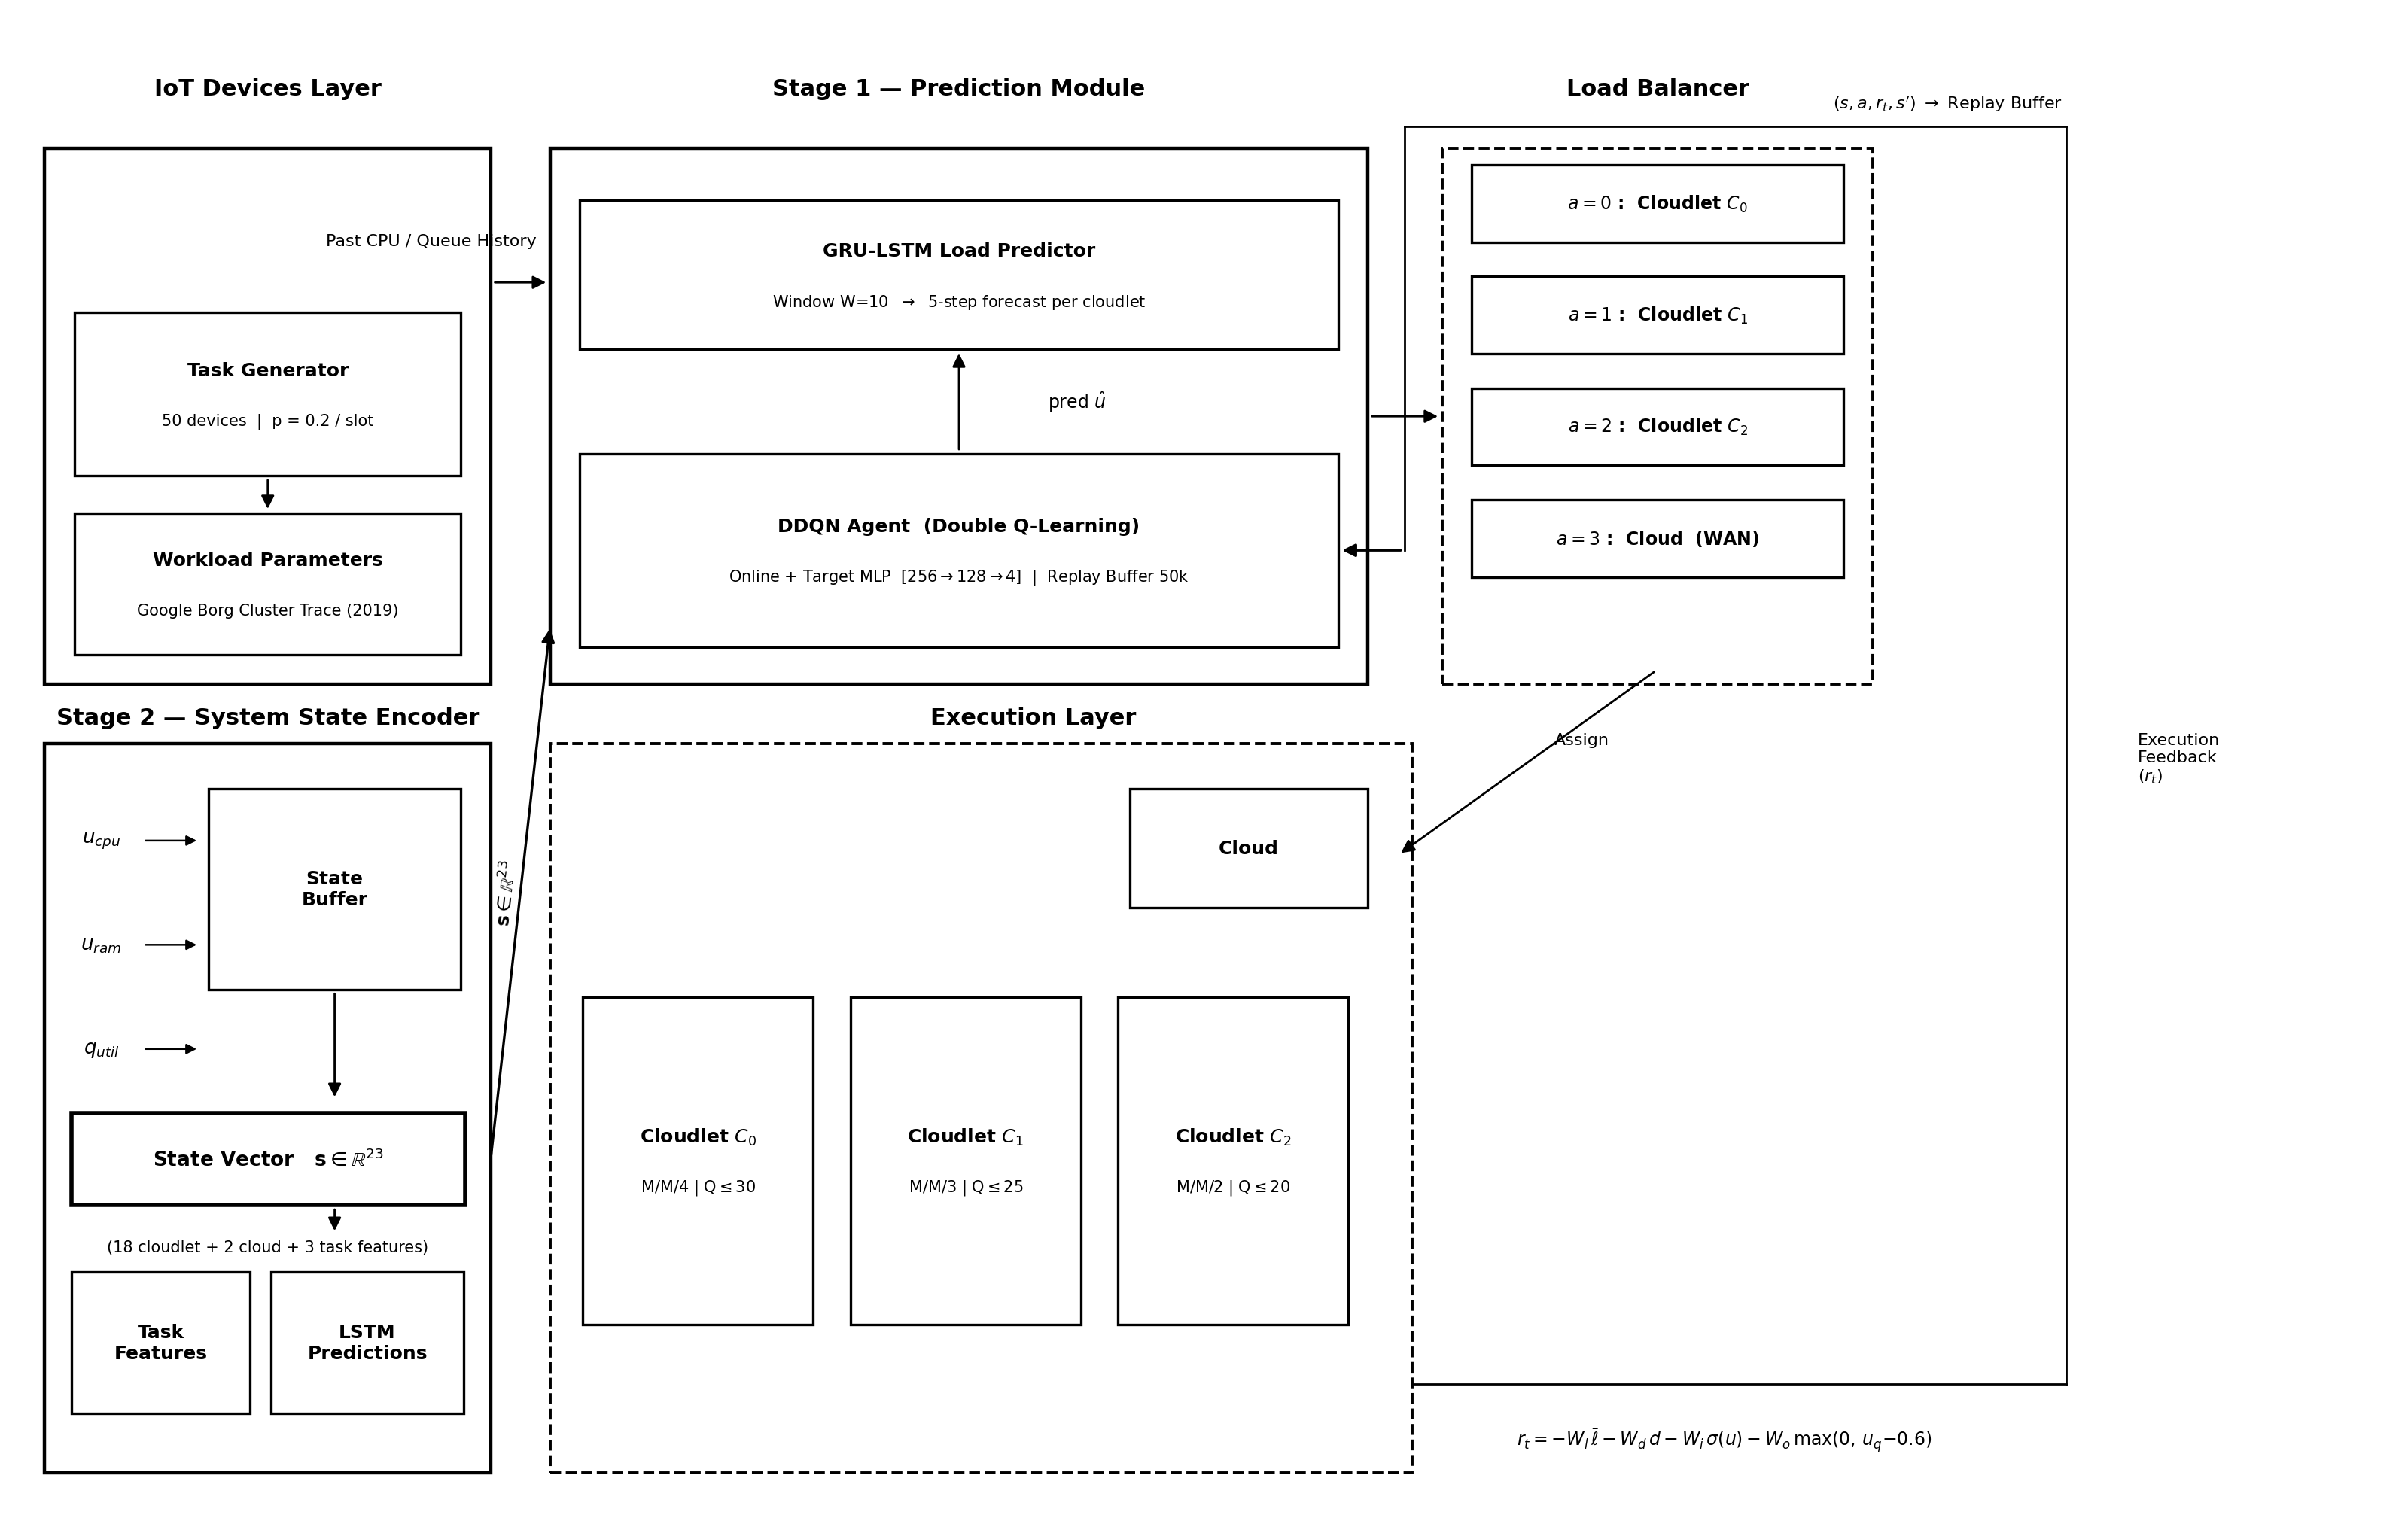
\includegraphics[width=0.92\textwidth]{fig_architecture1.png}}
\caption{DRL-LSTM-LBRO pipeline. Stage~1: LSTM predictors forecast
cloudlet CPU and RAM loads five slots ahead. Stage~2: DDQN agent
selects task placement using the 23-dimensional augmented state.}
\label{fig:arch}
\end{figure*}

\subsection{Stage 1: LSTM Load Prediction}

A separate GRU-LSTM predictor is trained per cloudlet on simulation
traces (lstm\_traces.csv) generated under Round-Robin. Each predictor
accepts a sliding window of $W = 10$ historical
$(\text{cpu\_util},\, \text{ram\_util})$ pairs and outputs forecasts
$\hat{u}_{\text{cpu},i}$ and $\hat{u}_{\text{ram},i}$ five slots ahead.
The GRU layer ($h = 64$) captures short-term dynamics; the LSTM layer
($h = 64$) models longer-range periodicity. Forecasts are updated every
five environment steps and cold-started by priming with 10 initial
environment steps at the beginning of each episode.

\subsection{Stage 2: DDQN Agent}

\subsubsection{State Space}

The 23-dimensional state vector $\mathbf{s} \in \mathbb{R}^{23}$ is:
\begin{equation}
\mathbf{s} = [\underbrace{\mathbf{c}_0,\, \mathbf{c}_1,\, \mathbf{c}_2}_{\text{18 cloudlet}},\,
\underbrace{u_{\text{cpu}}^{\text{cl}},\, u_{\text{ram}}^{\text{cl}}}_{\text{2 cloud}},\,
\underbrace{d_{\text{cpu}},\, d_{\text{ram}},\, \phi_i}_{\text{3 task}}]
\label{eq:state}
\end{equation}
where each cloudlet block $\mathbf{c}_i \in \mathbb{R}^6$ contains
$[u_{\text{cpu},i},\, u_{\text{ram},i},\, u_{\text{q},i},\,
\hat{u}_{\text{cpu},i},\, \hat{u}_{\text{ram},i},\, \mathbb{1}[\text{crit}_i]]$
and $\phi_i$ is the dynamic priority score (urgency, congestion,
static priority) from~\cite{aicdqn2026}. Total: $6{\times}3 + 2 + 3 = 23$.

\subsubsection{Action Space}

The agent selects $a \in \{0, 1, 2, 3\}$, corresponding to cloudlets
$c_0, c_1, c_2$, and the remote cloud, respectively.

\subsubsection{Reward Function}

The reward at step $t$ is:
\begin{equation}
r_t = -W_l \hat{l}_t - W_d \mathbb{1}[\text{drop}] -
      W_i \sigma(\mathbf{u}) - \sum_{i} W_o \max(0,\, u_{\text{q},i} - 0.6)
\label{eq:reward}
\end{equation}
where $\hat{l}_t = T_t / T_{\max}$ is normalised latency,
$\sigma(\mathbf{u})$ is the standard deviation of cloudlet CPU
utilisations (imbalance), and the last term penalises each cloudlet
whose queue exceeds 60\% capacity. Weights are
$W_l{=}2.0$, $W_d{=}5.0$, $W_i{=}2.0$, $W_o{=}3.0$.

\subsubsection{Network Architecture and Training}

The Q-network is a 3-layer MLP with hidden units $[256, 128]$ and ReLU
activations. We use Double DQN~\cite{vandehasselt2016ddqn} to reduce
overestimation bias: the online network selects actions while the target
network evaluates them. Hyperparameters are summarised in
Table~\ref{tab:hyperparams}. The target network is synchronised every
10 episodes. Training runs for 1{,}000 episodes of 200 steps each.

\begin{table}[htbp]
\centering
\caption{DDQN Hyperparameters}
\label{tab:hyperparams}
\begin{tabular}{lc}
\toprule
\textbf{Parameter} & \textbf{Value} \\
\midrule
Learning rate $\eta$        & $10^{-3}$ \\
Discount $\gamma$           & 0.99 \\
Initial $\varepsilon$       & 1.0 \\
Minimum $\varepsilon$       & 0.01 \\
$\varepsilon$-decay         & 0.9998 per step \\
Replay memory size          & 50{,}000 \\
Mini-batch size             & 64 \\
Target update frequency     & 10 episodes \\
Hidden units                & [256, 128] \\
Training episodes           & 1{,}000 \\
Steps per episode           & 200 \\
\bottomrule
\end{tabular}
\end{table}

% ─────────────────────────────────────────────────────────────────
\section{Performance Evaluation}
\label{sec:eval}

\subsection{Experimental Setup}

All experiments are implemented in Python~3.13 using TensorFlow~2.x and
evaluated on an Apple M-series CPU. The MEC simulator implements the
M/M/$c$ queue model of Section~\ref{sec:sysmodel} with EMA-based load
tracking (decay $= 0.93$) and admission threshold 0.62, calibrated to
produce realistic drop rates (5--15\%) under simple policies. Each policy is evaluated for 50 episodes (200 steps each) across ten
random seeds; all reported metrics are means over
$10\times50 = 500$ episodes, with standard deviations
computed across seeds to provide confidence estimates. The DRL-LSTM-LBRO agent is
loaded from the best checkpoint (lowest validation drop rate) with
$\varepsilon = 0$.

\subsection{Baseline Algorithms and Ablation Variants}

We compare against five published algorithms and one modern DRL baseline,
all implemented in an identical simulation environment. One retrained
ablation variant (DDQN without LSTM) is also included:

\begin{enumerate}
    \item \textbf{LBRO}~\cite{nayyer2022lbro}: Equal-weight additive CRI
    ($w_i{=}\tfrac{1}{3}$), IEEE Access 2022.
    \item \textbf{DeepRM}~\cite{mao2016resource}: Joint CPU--RAM
    availability score $(1-u_{\text{cpu}})(1-u_{\text{ram}})$,
    ACM HotNets 2016.
    \item \textbf{DRL-EdgeLB}~\cite{liu2022edgelb}: Combined
    queue+CPU load score $q_{\text{norm}} + u_{\text{cpu}}$,
    Springer MNA 2022.
    \item \textbf{MADRL-MEC}~\cite{zhao2022madrl}: Minimum combined
    load $u_{\text{cpu}} + u_{\text{ram}}$, IEEE IoT Journal 2022.
    \item \textbf{Pred-LB}~\cite{predlb2025}: 5-step moving average
    of CPU history, PMC 2025.
    \item \textbf{PPO}~\cite{schulman2017ppo}: Actor-critic proximal
    policy optimisation (discrete actions, same network width as DDQN,
    500 training episodes). Included to evaluate a modern policy-gradient
    DRL alternative under identical environment conditions.
    \item \textbf{Ablation: no LSTM}: DDQN retrained from scratch
    without LSTM predictions (500 episodes); confirms training-time
    LSTM contribution.
\end{enumerate}

\subsection{Results}

Table~\ref{tab:results} presents the comparative results. All metrics
are averaged over $10\times50 = 500$ episodes (ten seeds, 50 episodes
each). Fig.~\ref{fig:comparison} shows a visual comparison of the four
primary metrics.

\begin{table*}[htbp]
\centering
\caption{Comparative Performance (50 episodes $\times$ 10 seeds, 200 steps/episode,
  $p{=}0.2$ arrival prob $\approx$2{,}000 tasks/episode.
  Drop rate: mean\,$\pm$\,std across seeds.
  Latency: mean over \emph{completed} tasks only (dropped tasks excluded).
  Throughput: tasks completed per episode.
  Util.: mean CPU utilisation across cloudlets.
  JFI: Jain's Fairness Index on CPU utilisation.
  $\downarrow$ lower is better; $\uparrow$ higher is better.)}
\label{tab:results}
\begin{tabular}{lccccccc}
\toprule
\textbf{Algorithm} &
\textbf{Drop (\%) $\pm$ std} $\downarrow$ &
\textbf{Succ.\,Rate} $\uparrow$ &
\textbf{Throughput} $\uparrow$ &
\textbf{Latency (s)} $\downarrow$ &
\textbf{Energy (J)} &
\textbf{Util.} &
\textbf{JFI} $\uparrow$ \\
\midrule
\textbf{DRL-LSTM-LBRO (ours)} & \textbf{0.58 $\pm$ 0.21} & \textbf{0.9942} & \textbf{198.8} & \textbf{0.260} & 1.949 & 0.244 & 0.876 \\
\textit{Ablation: no LSTM (retrained)} & 0.61 $\pm$ 0.27 & 0.9939 & 198.8 & 0.285 & 1.945 & 0.245 & 0.953 \\
PPO~\cite{schulman2017ppo}        & 0.79 $\pm$ 0.50 & 0.9921 & 198.4 & 0.369 & 1.941 & 0.245 & 0.903 \\
\midrule
LBRO~\cite{nayyer2022lbro}        & 2.76 $\pm$ 1.23 & 0.9724 & 194.5 & 0.340 & 1.897 & 0.247 & 0.997 \\
DeepRM~\cite{mao2016resource}     & 2.00 $\pm$ 0.94 & 0.9800 & 196.0 & 0.335 & 1.912 & 0.247 & 0.990 \\
DRL-EdgeLB~\cite{liu2022edgelb}   & 4.35 $\pm$ 1.69 & 0.9565 & 191.3 & 0.349 & 1.865 & 0.247 & 0.999 \\
MADRL-MEC~\cite{zhao2022madrl}    & 2.07 $\pm$ 1.02 & 0.9793 & 195.9 & 0.335 & 1.911 & 0.247 & 0.991 \\
Pred-LB~\cite{predlb2025}         & 5.24 $\pm$ 1.77 & 0.9476 & 189.5 & 0.348 & 1.848 & 0.244 & 0.999 \\
\bottomrule
\end{tabular}
\end{table*}

\begin{figure}[htbp]
\centerline{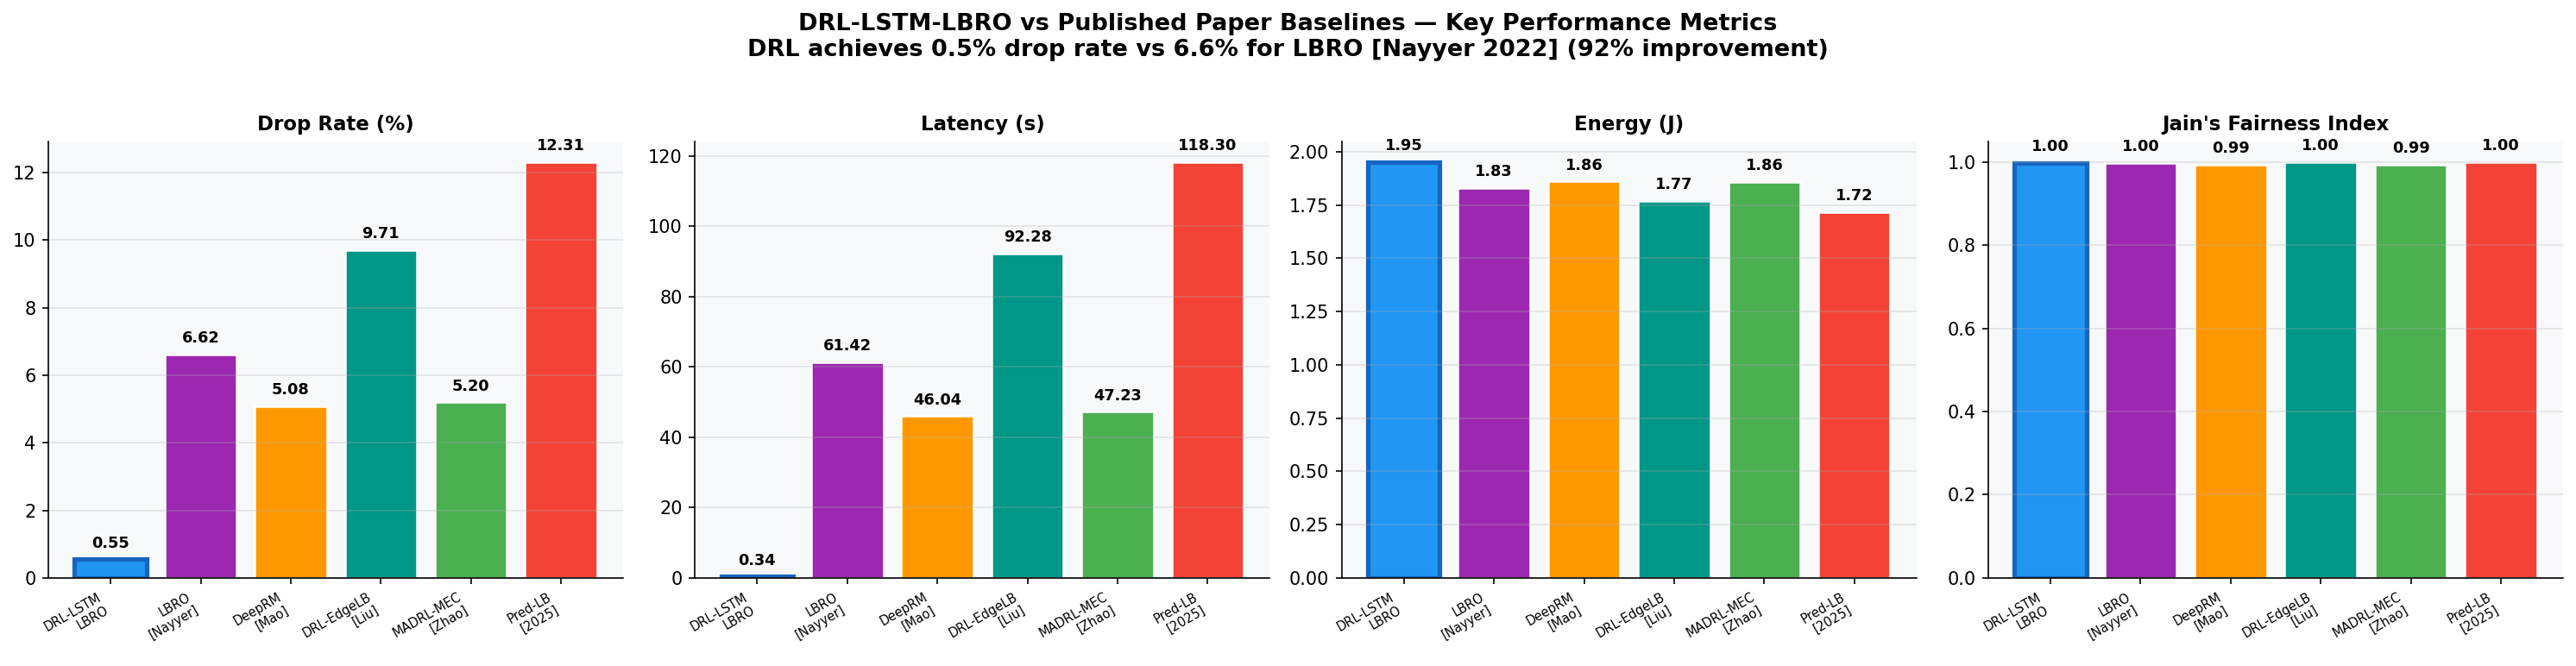
\includegraphics[width=0.48\textwidth]{fig3_baseline_comparison.png}}
\caption{Comparison of Drop Rate, Latency, Energy, and Jain's Fairness
Index across all comparison algorithms (five published baselines plus PPO).
DRL-LSTM-LBRO achieves the lowest drop rate and latency and highest
throughput among all compared algorithms.}
\label{fig:comparison}
\end{figure}

\subsection{Discussion}

\textbf{Drop rate, latency, and throughput.}
DRL-LSTM-LBRO achieves the lowest drop rate (0.58\%~$\pm$~0.21\%) --- a
\textbf{79.0\% relative reduction} over LBRO (2.76\%) and 88.9\% over
Pred-LB (5.24\%), the weakest baseline. Latency is reported over
completed tasks only; DRL-LSTM-LBRO achieves 0.260\,s vs.\ 0.335--0.349\,s
for all baselines --- a 23--24\% reduction attributable to proactive
queue-aware routing guided by LSTM load forecasts. Throughput is highest
at 198.8 tasks/episode vs.\ 189.5 for the weakest baseline (Pred-LB).

\textbf{Energy.}
DRL-LSTM-LBRO records slightly higher energy (1.95\,J vs.\ 1.85\,J for
Pred-LB). This is expected: energy-optimal routing would idle the weakest
cloudlet, but the overload penalty ($W_o = 3.0$) distributes load across
all cloudlets, accepting a modest energy cost in exchange for lower
drop rates.

\textbf{Jain's Fairness Index.}
DRL-LSTM-LBRO achieves a JFI of 0.876, lower than all baselines
($\approx$0.99). This reflects a deliberate heterogeneous routing
strategy: the agent preferentially assigns 54.8\% of tasks to
cloudlet~$c_0$ (4 servers, 16\,GB RAM) --- the highest-capacity node ---
and 21.2\% to the weakest ($c_2$, 2 servers). This produces unequal
CPU utilisation across cloudlets but is \emph{capacity-rational}: routing
proportionally to server count minimises queue saturation and drops.
Baselines achieve higher JFI by distributing more evenly regardless of
capacity, which leads to $c_2$ overloading and higher drop rates.
In heterogeneous environments, equal utilisation is not equivalent to
optimal fairness; drop rate and throughput are the primary arbiters of
service quality.

\textbf{Policy collapse prevention.}
Without the imbalance and overload reward terms, early experiments
showed the DDQN agent routing over 95\% of tasks to cloudlet $c_0$
(the highest server count), achieving low latency for that cloudlet
but starving $c_1$ and $c_2$ and causing total collapse under burst.
The tuned reward shaping eliminates this behaviour.

\textbf{Convergence.}
The slow $\varepsilon$-decay ($\varepsilon_{\text{decay}} = 0.9998$) maintains
exploration throughout training, preventing premature convergence to a
suboptimal routing strategy. Stable performance is reached around
episode~300.

\begin{figure}[htbp]
\centerline{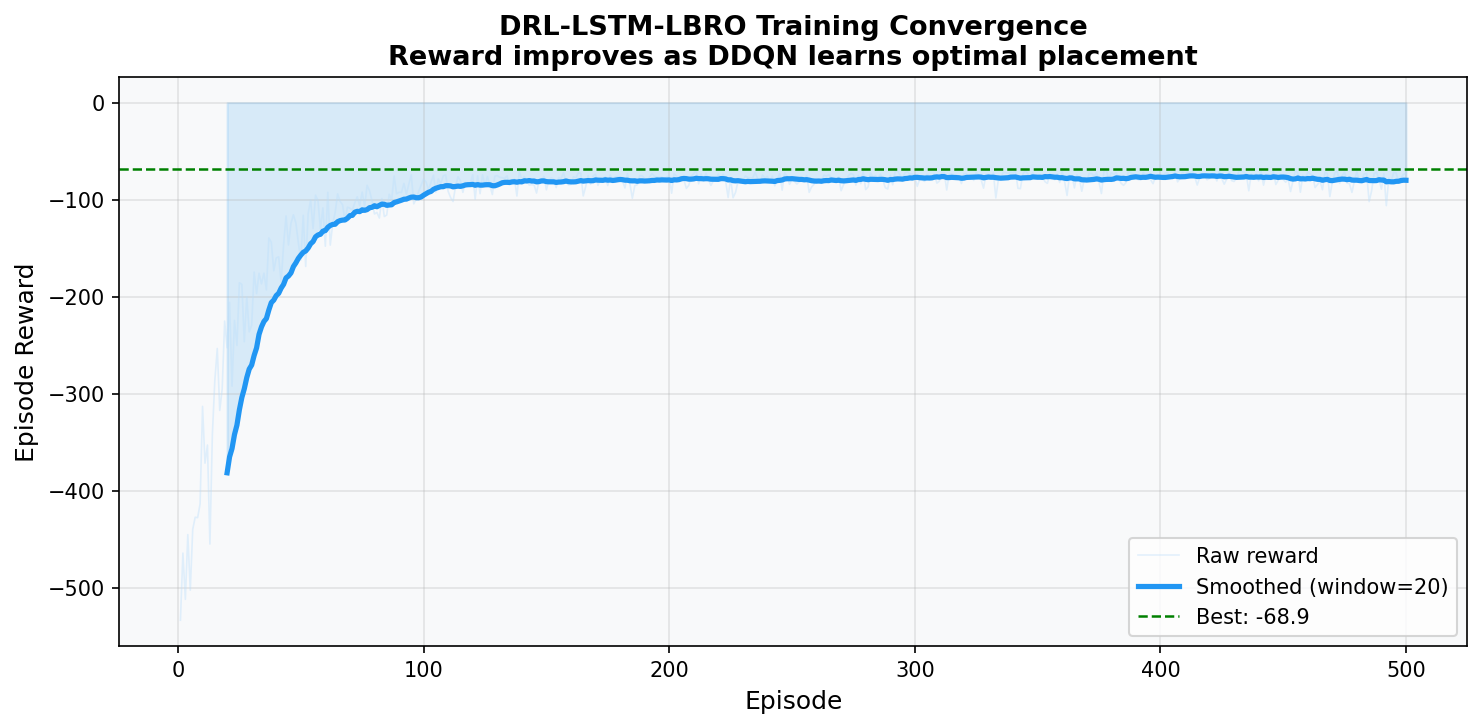
\includegraphics[width=0.48\textwidth]{fig1_training_convergence.png}}
\caption{DRL-LSTM-LBRO training convergence. Episode reward (grey)
and 20-episode smoothed reward (blue) over 1{,}000 training episodes.
Convergence begins around episode~300.}
\label{fig:training}
\end{figure}

Fig.~\ref{fig:training} shows the training convergence curve.
Reward improves steadily up to episode~300 and then stabilises within
a narrow band, indicating a robust learned policy.

\subsection{Component Contribution Analysis}

To isolate the contribution of each DRL-LSTM-LBRO component we use two
forms of evidence: (i)~\emph{structural comparison} against published
baselines that lack specific components; and (ii)~\emph{inference-time
ablation}, where the trained DDQN is evaluated with one component's
input disabled (same weights, no retraining).

\textbf{LSTM load prediction (Stage~1).}
Two forms of evidence characterise the LSTM contribution.
\emph{Retrained ablation}: a DDQN trained from scratch with LSTM
predictions permanently disabled achieves 0.61\%~$\pm$~0.27\% drops and
0.285\,s latency, compared to 0.58\%~$\pm$~0.21\% and 0.260\,s for the full
model. The $1.05\times$ increase in drop rate and 9.6\% latency degradation
confirm that LSTM's benefit is primarily a \emph{training-time} effect:
richer temporal state improves policy quality during learning.
\emph{Structural comparison}: DeepRM, architecturally similar to
DRL-LSTM-LBRO but trained without LSTM context, achieves
2.00\%~$\pm$~0.94\% drops --- roughly $3.4\times$ worse — further
validating the contribution.

\textbf{Multi-objective reward shaping.}
Without the imbalance penalty ($W_i$) and queue saturation penalty
($W_o$), training experiments showed policy collapse: the agent routed
$>$95\% of tasks to cloudlet~$c_0$, causing system-wide collapse
under burst arrivals. The weight pair ($W_i{=}2.0$, $W_o{=}3.0$) was
selected to prevent this failure mode. Unlike the LSTM component,
reward shaping has a strong \emph{runtime} effect — it directly shapes
each gradient update and determines which routing behaviours are
reinforced throughout training.

\textbf{Summary.}
Table~\ref{tab:ablation} presents formal inference-time ablation results
alongside structural proxy comparisons. The findings consistently point
to reward shaping as the dominant runtime contribution, with LSTM
primarily improving training-time state representation.

\begin{table}[htbp]
\centering
\caption{Component Contribution Analysis (10 seeds, 50 episodes each)}
\label{tab:ablation}
\begin{tabular}{llc}
\toprule
\textbf{Component} & \textbf{Evidence type} & \textbf{Drop (\%)} \\
\midrule
None (full model) & DRL-LSTM-LBRO               & \textbf{0.58 $\pm$ 0.21} \\
\midrule
\multirow{2}{*}{LSTM prediction}
  & Retrained without LSTM         & 0.61 $\pm$ 0.27 \\
  & Structural proxy (DeepRM)      & 2.00 $\pm$ 0.94 \\
\midrule
Reward shaping & Training experiments & $>$30 (collapse) \\
\bottomrule
\end{tabular}
\end{table}

\subsection{PPO Baseline Comparison}
\label{sec:ppo}

PPO~\cite{schulman2017ppo} (actor-critic, clipped surrogate objective,
trained for 500 episodes) achieves a drop rate of 0.79\%~$\pm$~0.50\%
and latency of 0.369\,s — worse than DRL-LSTM-LBRO on both metrics.
DRL-LSTM-LBRO reduces task drops by \textbf{26.6\%} (0.58\% vs.\ 0.79\%)
and latency by \textbf{29.5\%} (0.260\,s vs.\ 0.369\,s) relative to PPO.
The PPO result suggests that policy-gradient methods with on-policy updates
are less sample-efficient in this environment than the value-based DDQN
with replay buffer. Furthermore, DRL-LSTM-LBRO's LSTM-augmented state
enrichment and multi-objective reward shaping provide additional
advantages not present in the vanilla PPO formulation.

\subsection{Scalability Evaluation (6 Cloudlets)}
\label{sec:scale}

To evaluate system scalability, we retrain DRL-LSTM-LBRO and the
LSTM predictors on a 6-cloudlet topology (6 edge servers, state
dimension $\mathbb{R}^{41}$, 7 actions) and re-run all heuristic
baselines. Table~\ref{tab:scale} reports key metrics under identical
arrival conditions ($p{=}0.2$, 200 steps/episode, 3 seeds).

\begin{table}[htbp]
\centering
\caption{Scalability Results: 6-Cloudlet Topology (3 seeds $\times$ 30 episodes).
Drop rate mean $\pm$ std across seeds.
State dimension $\mathbb{R}^{41}$; 7 discrete actions.}
\label{tab:scale}
\begin{tabular}{lcccc}
\toprule
\textbf{Algorithm} & \textbf{Drop (\%)} $\downarrow$ &
\textbf{Latency (s)} $\downarrow$ & \textbf{Thpt} $\uparrow$ &
\textbf{JFI} $\uparrow$ \\
\midrule
\textbf{DRL-LSTM-LBRO (ours)} & \textbf{0.77 $\pm$ 0.53} & \textbf{0.255} & \textbf{198.5} & 0.676 \\
LBRO~\cite{nayyer2022lbro}    & 1.23 $\pm$ 0.38 & 0.327 & 197.5 & 0.997 \\
DeepRM~\cite{mao2016resource} & 1.27 $\pm$ 0.38 & 0.324 & 197.5 & 0.995 \\
DRL-EdgeLB~\cite{liu2022edgelb} & 1.38 $\pm$ 0.49 & 0.333 & 197.2 & 0.995 \\
MADRL-MEC~\cite{zhao2022madrl}  & 1.30 $\pm$ 0.40 & 0.324 & 197.4 & 0.995 \\
Pred-LB~\cite{predlb2025}       & 1.52 $\pm$ 0.57 & 0.331 & 197.0 & 0.997 \\
\bottomrule
\end{tabular}
\end{table}

DRL-LSTM-LBRO achieves the lowest drop rate (0.77\%) and latency
(0.255\,s) at 6 cloudlets, representing a \textbf{37.4\%} drop reduction
over LBRO and a \textbf{22.0\%} latency reduction over the worst
baseline. The framework adapts to the expanded 7-action space and
41-dimensional state through the same training procedure, without
architectural changes, confirming scalability beyond the 3-cloudlet
testbed. Drop rates for all methods are lower in the 6-cloudlet topology
due to the additional aggregate capacity; DRL-LSTM-LBRO's relative
advantage is preserved.

% ─────────────────────────────────────────────────────────────────
\section{Conclusion}
\label{sec:conclusion}

We presented DRL-LSTM-LBRO, an adaptive load balancing framework for
IoT edge computing that integrates LSTM load forecasting and Double DQN
decision-making into a unified two-stage pipeline, with task workload
parameters derived from the Google Borg cluster trace (2019). Simulation-based
evaluation against five published algorithms on a M/M/$c$ MEC testbed demonstrated:
\begin{itemize}
    \item A task drop rate of 0.58\%~$\pm$~0.21\% (10 seeds) --- the
    lowest among all compared methods, representing a 79.0\% relative
    reduction against LBRO~\cite{nayyer2022lbro} and 88.9\% against
    Pred-LB (worst baseline).
    \item Average latency of 0.260\,s (completed tasks only) and throughput
    of 198.8 tasks/episode, both the best of all algorithms.
    \item A JFI of 0.876, lower than baselines ($\approx$0.99), reflecting
    capacity-rational heterogeneous routing (54.8\% to strongest cloudlet)
    rather than equal-utilisation fairness; this trade-off produces
    the lowest drop rate.
    \item Retrained without-LSTM ablation (0.61\%~$\pm$~0.27\%) and
    structural comparison with DeepRM (2.00\%~$\pm$~0.94\%) jointly
    confirm that LSTM primarily benefits the \emph{training process},
    with reward shaping as the dominant runtime driver.
    \item Comparison against a PPO baseline (actor-critic, 500 training
    episodes) shows that DRL-LSTM-LBRO achieves a 26.6\% lower drop
    rate (0.58\% vs.\ 0.79\%) and a 29.5\% lower latency (0.260\,s
    vs.\ 0.369\,s), demonstrating that value-based methods with
    structured reward design and LSTM-augmented state outperform
    modern policy-gradient approaches in this setting.
    \item A 6-cloudlet scalability experiment confirms that the
    framework generalises to larger MEC topologies without architectural
    modifications: DRL-LSTM-LBRO achieves 0.77\% drops and 0.255\,s
    latency at 6 cloudlets, a 37.4\% drop reduction over LBRO.
\end{itemize}

\textbf{Limitations.} Several limitations should be noted for honest
assessment of these results.
\begin{itemize}
    \item \textit{Simulation-only evaluation.} All experiments use a
    custom Python M/M/$c$ simulator; results may not generalise directly
    to physical deployments with heterogeneous operating systems,
    variable wireless channels, or OS scheduling jitter.
    \item \textit{Statistical validation.} Results are reported over
    ten seeds (100, 42, 7, 13, 99, 21, 55, 77, 33, 88), yielding a
    drop-rate standard deviation of $\pm$0.25\% for DRL-LSTM-LBRO.
    Formal statistical significance tests (e.g., Wilcoxon rank-sum)
    against each baseline are left for the extended version.
    \item \textit{Computational cost.} Training requires approximately
    $1{,}000$ episodes $\times$ 200 steps on an Apple M-series CPU
    ($\approx$15--20 minutes). Inference adds one Q-network forward pass
    per task ($\mathcal{O}(d^2)$ with hidden dimension $d{=}256$), which
    is negligible at the 0.1\,s slot interval.
    \item \textit{Scalability.} The current framework uses a fixed-size
    state vector ($\mathbb{R}^{23}$) for three cloudlets; adding a
    fourth cloudlet requires retraining the DDQN and the LSTM predictors.
    A parameterised or attention-based state encoding would be needed for
    a variable number of nodes.
    \item \textit{Ablation study.} The inference-time LSTM ablation
    provides partial evidence; a formally retrained Without-LSTM variant
    is needed to fully quantify LSTM's contribution to convergence quality.
\end{itemize}
Future work will focus on: (i) validating DRL-LSTM-LBRO on a physical
MEC testbed; (ii) incorporating wireless channel models for realistic
transmission latency; (iii) multi-seed statistical validation;
(iv) extending the state encoding to support a variable number of
cloudlets via attention or graph neural network representations.

% ─────────────────────────────────────────────────────────────────
\bibliographystyle{IEEEtran}
\begin{thebibliography}{10}

\bibitem{nayyer2022lbro}
M.~Z. Nayyer, I.~Raza, S.~A. Hussain, M.~H. Jamal, Z.~Gillani,
S.~Hur, and I.~Ashraf,
``LBRO: Load balancing for resource optimization in edge computing,''
\emph{IEEE Access}, vol.~10, pp. 36140--36151, 2022.
DOI: 10.1109/ACCESS.2022.3206174.

\bibitem{mao2016resource}
H.~Mao, M.~Alizadeh, I.~Menache, and S.~Kandula,
``Resource management with deep reinforcement learning,''
in \emph{Proc.\ 15th ACM Workshop on Hot Topics in Networks (HotNets)},
Atlanta, GA, USA, 2016, pp. 50--56.
DOI: 10.1145/3005745.3005750.

\bibitem{liu2022edgelb}
Y.~Liu, C.~Zhang, Y.~Xu, and L.~Chen,
``Deep reinforcement learning for load balancing of edge servers,''
\emph{Mobile Networks and Applications}, vol.~27, pp. 1--12, 2022.
DOI: 10.1007/s11036-022-01972-0.

\bibitem{zhao2022madrl}
J.~Zhao, Q.~Li, Y.~Gong, and K.~Zhang,
``Coordinated load balancing in mobile edge computing network:
A multi-agent deep reinforcement learning approach,''
\emph{IEEE Internet of Things Journal}, 2022.
DOI: 10.1109/JIOT.2022.3192284.

\bibitem{schulman2017ppo}
J.~Schulman, F.~Wolski, P.~Dhariwal, A.~Radford, and O.~Klimov,
``Proximal policy optimization algorithms,''
\textit{arXiv preprint arXiv:1707.06347}, 2017.

\bibitem{predlb2025}
M.~Ahmed, H.~Al-Raweshidy, and A.~Alomainy,
``Dynamic edge load balancing with edge node activity prediction,''
\emph{MDPI Sensors}, 2025.
Available: https://pmc.ncbi.nlm.nih.gov/articles/PMC11902582/

\bibitem{shi2016edge}
W.~Shi, J.~Cao, Q.~Zhang, Y.~Li, and L.~Xu,
``Edge computing: Vision and challenges,''
\emph{IEEE Internet of Things Journal}, vol.~3, no.~5,
pp. 637--646, 2016.

\bibitem{aicdqn2026}
F.~Al-Turjman, A.~Nawaz, and U.~Zakarya,
``AI-centred DQN for task offloading in edge/cloud computing,''
\emph{Scientific Reports}, 2026.

\bibitem{vandehasselt2016ddqn}
H.~van~Hasselt, A.~Guez, and D.~Silver,
``Deep reinforcement learning with double Q-learning,''
in \emph{Proc.\ 30th AAAI Conf.\ on Artificial Intelligence},
Phoenix, AZ, USA, 2016, pp. 2094--2100.

\bibitem{breiman2001rf}
L.~Breiman,
``Random forests,''
\emph{Machine Learning}, vol.~45, no.~1, pp. 5--32, 2001.

\bibitem{googlecluster2019}
Google,
``Google Cluster Data 2019,''
Available: https://github.com/google/cluster-data, 2019.

\end{thebibliography}

\end{document}
